L'apprendimento automatico (o \textit{Machine Learning}) è una branca dell'informatica basata sull'idea di pemettere ai computer di imparare da esempi e include tecniche, dalla semplice ricerca locale alle \textit{support vector machines}. 
 Le reti neurali sono una tecnica di \emph{machine learning} ma non sono l'unica esistente anche se al momento stanno avendo ampio successo. In questa relazione vedremo come sono nate, da cosa hanno tratto ispirazione e avremo una rapida scorsa su alcune delle tipologie più popolari. Analizzeremo più nello specifico come avviene l'apprendimento da parte delle reti e come siano state migliorate nel corso del tempo. Infine prenderemo in analisi vantaggi e svantaggi dei principali framework che le implementano.

\section{L'ispirazione biologica}
%\vspace{-2cm}
Il cervello umano è composto da circa 86 miliardi di neuroni e un numero totale di collegamenti fra loro di $10^{14}$. Nella figura \ref{biologia-neuroni} attorno al nucleo di colore verde si estende il corpo cellulare delle cellule neurali, dette \textit{soma}, e i canali di input ed output che la circondano la collegano a circa altri 10000 neuroni.
Ogni neurone riceve degli stimoli elettrochimici dai neuroni circostanti attraverso i proprio dendriti. Se la somma degli input elettrici è sufficientemente elevata il neurone trasmette a sua volta un segnale elettrochimico lungo l'assone, che viene diffuso a tutti quei neuroni i cui dendriti sono connessi alle terminazione del neurone in oggetto.
Per quel che vedremo in seguito è importante sottolineare come il neurone attivi il segnale in uscita solo se la totalità dei segnali in ingresso raggiunge un certo livello, a quel punto il neurone propaga il proprio impulso, senza sfumature di attivazione, o il segnale in uscita viene propagato o non viene propagato, non esistono segnali di potenza variabile da distribuire verso i neuroni connessi.
Il nostro intero cervello è quindi composto interamente da questa fitta rete di cellule, i neuroni, che comunicano fra loro attraverso segnali elettrochimici. \`E sorprendente vedere come la struttura alla base molto semplice, costituita da una cellula che a seconda della somma dei segnali in ingresso si attiva, o meno, comunicando con altre cellule attraverso segnali in uscita, riesca nel suo complesso reticolo di interazioni a svolgere funzioni complicate come quelle del cervello nella sua totalità.
Lo studio del cervello e la sua comprensione ha potuto ispirare i modelli scientifici e matematici che danno vita a quelle che sono dette \textit{reti neurali artificiali (in inglese \textit{Artificial Neural Networks}, ANN)}.
\clearpage

\vspace{2 cm}

\begin{figure}[b]
\centering
{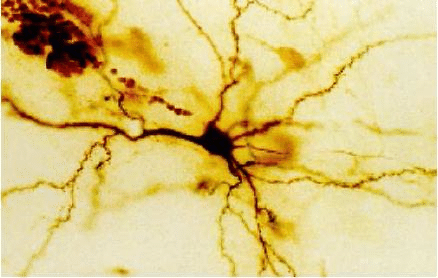
\includegraphics[scale=0.65]{media_tesi/real_neuron.png}}
\caption{Un immagine di un neurone ottenuta al microscopio da John Anderson, Institute for Neuroinformatics, Zurigo, Svizzera.}
\label{fig:subfig}
\end{figure}


\begin{figure}[h]
\centering
{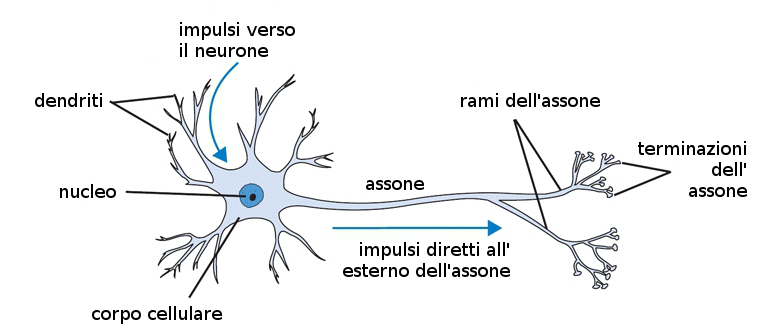
\includegraphics[scale=0.55]{media_tesi/neuron_model.png}}
\caption{Un modello di neurone biologico}
\label{biologia-neuroni}
\end{figure}

%
%\begin{figure}
%
%\centering
%
%\subfloat[][\emph{An impression of a real neuron. This image is a light microscope photograph by John Anderson, Institute for Neuroinformatics, Zurich, Switzerland.  }]
%{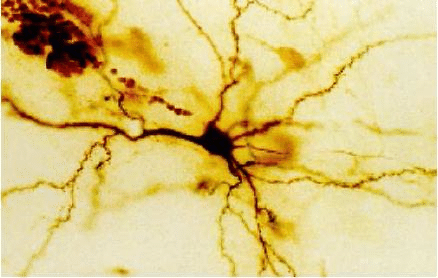
\includegraphics[width=.85\textwidth]{media_tesi/real_neuron.png}} \\
%
%
%\subfloat[][\emph{A biological neuron model}]
%{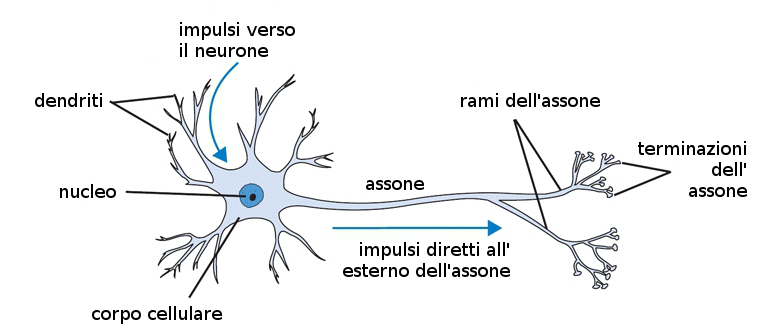
\includegraphics[width=.95\textwidth]{media_tesi/neuron_model.png}} \\
%
%\label{biologia-neuroni}
%\end{figure}
%
%\begin{figure}
%	\centering
%\end{figure}
\clearpage

\section*{La storia delle reti neurali}
Le prime forme di apprendimento autonomo si svilupparono inizialmente come il tentativo di due scienziati di  comprendere meglio il funzionamento dei nuroni nel cervello.
Era il 1943 e il neurofisiologo Warrent McCulloch e il matematico Walter Pitts ipotizzarono, per via della natura discreta dei neuroni che sono o accesi o spenti, di poter descrivere gli eventi neurali attraverso la logica proposizionale e quindi di poterli implementare artificialmente con dei circuiti elettrici \cite{mcculloch1943logical}.
Nel 1949 Donald Hebb scrisse \textit{L'organizzazione del Comportamento} in cui affermava di come i percorsi neurologici tendessero a rinforzarsi e a diventare più solidi mano mano che questi venivano allenati e utilizzati \cite{hebb1961organization}. Un lavoro che troverà conferme in studi successivi e documentati nel saggio di Nicholas Carr del 2010, in cui si fa riferimento alla plasticità del nostro cervello e alla capacità dei nostri neuroni di rinforzare i loro collegamenti man mano che vengono ``allenati'', similmente a un fiume, come riporta Carr stesso: \emph{"L'acqua che scorre solca un canale che si fa sempre più ampio e profondo; e quando l'acqua vi scorre di nuovo, segue con più facilità il percorso già tracciato in precedenza"} \cite{carr2010shallows}.
Nel frattempo i calcolatori diventavano più potenti e sul finire degli anni '50 Bernard Widrow e Marcian Hoff della Stanford University svilupparono ``ADALINE'' and ``MADALINE'' \cite{widrow1960adaptive}. La prima era in grado di riconoscere dei pattern binari nel linee telefoniche e predire i successivi bit in ingresso; la seconda fu la prima rete neurale ad essere applicata in un problema del mondo reale, ovvero era in grado, grazie a dei filtri adattivi, di eliminare gli echi nel chiamate al telefono. Questo dispositivo, per quanto datato e primitivo, funziona così bene da avere ancora oggi una sua validità commerciale.
Nel corso degli anni, nonostante i primi buoni risultati delle reti neurali, l'architettura di von Neumann si impose sulla scena dello sviluppo dei calcolatori, nonostante von Neumann stesso suggerisse di apprezzare l'approccio dell'imitazione delle funzionali neurali \cite{stanford_history}.
Il lavoro di Minsky e Papert, due professori del MIT, mostrò i limiti dell'apprendimento del perceptrone e delle reti neurali a singolo strato, portando i più ad abbandonare questo ramo della ricerca\cite{minsky2017perceptrons}. Gli iniziali successi condussero ad esagerare potenziale ed aspettative nei confronti delle reti neurali, generando in un primo momento clamore e diffidenza, paura anche rispetto a quallo che avrebbe potuto costituirsi come rapporto uomo-macchina e in seguito in delusione verso le aspettative non ripagate. 
Nel 1972 furono sviluppate indipendentemente da Kohonen e Anderson delle reti molto simili che si basavano su una memoria associativa\cite{kohonen1972correlation}; del 1975 è invece la prima rete multistrato non supervisionata.

L'interesse verso le reti neurali artificiali si rinnovò nel 1982 quando  John Hopfield della Caltech (USA) presentò un paper all'Accademia Nazionale delle Scienze \cite{hopfield1982neural}. In questo documento presentava l'opportunità di rendere le macchine più utili ed efficienti usando reti bidirezionali rompendo con la tradizionale idea di reti in cui i sengali si propagassero in un'unica direzione. Nello stesso anno altri due ricercatori: Reilly e Cooper usarono reti ``ibiride'' che applicavano differenti strategie di risoluzione per ognuno dei diversi strati della loro rete\cite{reilly1982neural}. Ancora nel 1982 una spinta ai finanziamenti in questo settore arrivò da una conferenza congiunta tra studiosi statunitensi e giapponesi sul tema. Vedendo i nipponici in vantaggio sullo sviluppo di queste tecnologie gli americani decisero di aumentare le risorse a disposizione della ricerca.

Nel 1986 arriviamo ad una svolta che diventa centrale nel corso di questa relazione, ovvero, lo sviluppo dell'idea del backpropagation error. Tre gruppi indipendenti di sviluppatori, tra i quali compariva David Rumelhart, un ex professore di Stanford del dipartimento di psicologia, arrivarono sempre indipendentemente all'idea  di distribuire gli errori prodotti dalla computazione della rete su tutta la rete stessa in modo da riprogrammarne i parametri e farla apprendere dai propri errori\cite{rumelhart1985learning}.
Quelle che prima abbiamo chiamato reti ``ibiride'' avevano solo due layer mentre queste nuove reti a retropropagazione dell'errore presentavano molti livelli e, dato lo stato dell'arte degli hardware del tempo, erano ritenute molto lente; e così hanno proseguito ad essere, tanto che negli anni 2000, le computazioni potevano richiedere settimane intere. Così è stato finché i recenti sviluppi degli ultimi anni hanno messo a disposizione delle reti hardware performanti e notevoli quantità di dati da cui le reti possano trarre informazioni ed imparare \cite{stanford_history}.

\section{I diversi tipi rete neurale}
Al giorno d'oggi le reti neurali sono tante e diverse tra loro; in questa sezione ne vedremo alcune delle principali tipologie. Qui verranno presentati brevemente solo i modelli principali, per un overview più esaustivo si veda \cite{networks_zoo}.
Le reti neurali biologiche hanno ispirato le reti neurali artificiali che vengono utilizzate per approssimare delle funzioni che non sono conosciute a priori \cite{wiki:tipi} e questo costituisce, semplicisticamente, un ribaltamento del classico paradigma con cui usiamo i computer: la programmazione infatti usa funzioni impostate dal programmatore per computare dei dati in output mentre le reti neurali cercano di creare una funzione a partire da dati forniti.
Le reti feedforward furono le prime reti ad essere pensate e sono anche le più semplici. Sono costituite da diversi strati (\textit{layers}), che possono essere di input per i dati di apprendimento, nascosti o di output.
Il perceptrone può essere visto come modello di un neurone biologico e può approssimare nella sua semplicità dei circuiti logici. Gli strati delle feed-forward sono tutti collegati fra loro e il flusso dei dati viaggia in una sola direzione, senza mai formare cicli, dallo strato di input, attraverso gli strati nascosti fino allo strato di output. Questa rete viene definita profonda all'aumentare degli \textit{hidden layers} che si nascondono fra input ed output e prendono il nome di \textit{deep feedforward neural networks}. Il numero di livelli nascosti oltre il quale una rete si definisce profonda varia a seconda del contesto: da più di uno ad oltre 10.


\begin{figure}[hbtb]
\centering
\subfloat[][\emph{un perceptrone}]
{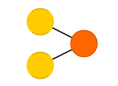
\includegraphics[scale=1.3]{media_tesi/perceptron.png}} \quad
\subfloat[][\emph{una FF}]
{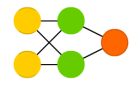
\includegraphics[scale=1.3]{media_tesi/feed_forward.png}} \quad
\subfloat[][\emph{una DFF}]
{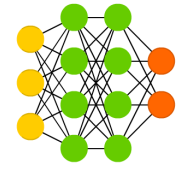
\includegraphics[scale=0.8]{media_tesi/DFF.png}}\\

\label{fig:subfig}
\end{figure}

Esistono poi anche le \textit{radial basis network} (RBF) che altro non sono che reti feedforward (e che possiamo schematizzare proprio come la FF in figura sopra) ma con una funzione di attivazione radiale di base. Non tutte le reti prendono il nome dalla propria funzione di attivazione ma questa sembrava avere particolari speranze nel 1988, quando uscì il documento che la presentava poiché la funzione che stava alla sua base era in grado di interpolare in spazi di molte dimensioni\cite{broomhead1988radial}.
 
%------------------------------------------
%\begin{wrapfigure}{R}{7.0cm}
%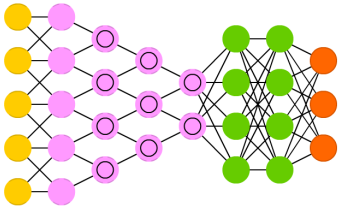
\includegraphics[scale=0.7]{media_tesi/DCN.png}
%\caption{Una DCN}\label{wrap-fig:1}
%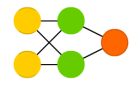
\includegraphics[scale=1.4]{media_tesi/feed_forward.png}
%\caption{rete convoluzionale profonda (DCN).}\label{wrap-fig:1}
%\end{wrapfigure} 
%------------------------------------------
Un altro caso speciale o un evoluzione delle FF sono le \textit{reti convoluzionali profonde} (\textit{deep convolutional network , DCN}) il cui utilizzo primario è il processing delle immagini e in alcuni casi anche degli input audio \cite{lecun1998gradient}. Si ispirano a quelle che è il funzionamento del sistema visivo degli uomini.
Le reti convoluzionali sono in grado di riconoscere soggetti nelle immagini sapendo quindi fare una classificazione in un insieme di immagini che gli vengono sottoposte. Le DCN scansionano le immagini partendo da piccoli blocchi di pixel vicini tra loro e individuano le caratteristiche delle immagini porzione dell'immagine per porzione, fino a classificare l'immagine nella sua totalità.
Diversamente delle tradizionali feed-forward i layer di mezzo non sono completamente connessi, piuttosto i nodi vicini sono collegati ad un intorno dei nodi vicini nello strato successivo. Questo vuole ispirarsi al modo in cui il nostro campo visivo funziona e reagisce agli stimoli esterni. Man mano che il segnale fluisce lungo la rete attraversa strati costituiti da sempre meno nodi fino ad arrivare alla terminazione della rete in cui viene ``attaccata'' una piccola rete FF che consente di processare ulteriormente i dati e fare nuove astrazioni.

Un recente sviluppo, del 2014, delle reti che sembra essere promettente è la combinazione di due reti insieme. Di solito vengono associate tra loro FF e reti convoluzionali e si impostano in modo tale che esse si contrappongano nello svolgere dei compiti. Immaginiamo un pittore che dipinge su una tela un gatto, in sua compagnia un giudice verifica la qualità del lavoro confrontandolo che un insieme di fotografie di gatti reali; il pittore si allena a ritrarre sempre più fedelmente i gatti e il giudice viene sfidato nel giudicare via via se il gatto sottopostogli dall'amico sia una fedele riproduzione artistica o una foto reale. Ecco nelle \emph{generative adversarial networks} (\textit{GAN}) una delle due reti fa un lavoro di generazione mentre l'altra fa un lavoro di giudizio, in pratica una genera contenuti che vengono giudicati dall'altra e si allenano vicendevolmente nel giudicare una l'operato dell'altra, spingendo la seconda a produrre contenuti sempre più difficili da predire mentre la prima viene allenata dalla seconda, che producendo via via lavori sempre più approssimabili a quelli dell'insieme di confronto \cite{goodfellow2014generative}.

Abbiamo parlato fin'ora solamente di reti in cui i segnali partendo da uno strato di input si propagano unidirezionalmente verso la fine della rete. \`E giusto ricordare brevemente anche quelle reti che invece formano dei cammini ciclici fra i loro nodi.

Le \emph{Recurrent Neural Networks (RNN)} sono delle reti feed-forward in cui il flusso di dati non procede soltanto in una direzione ma i valori di uscita in un livello posson essere usati come input per uno strato ad esso inferiore \cite{elman1990finding}. Questa interconnessione permette alla rete di conservare le informazioni in una memoria di stato. Questo le rende appetibili in quelle applicazioni dove la sequenza temporale in cui dei dati vengono registrati è importante: ad esempio l'analisi predittiva dei prezzi di borsa, la previsione della prossima parola inserita in un editor di testo o il riconoscimento vocale \cite{rrn-medium}.

\begin{figure}[hbtb]
\centering
\subfloat[][\emph{una DCN}]
{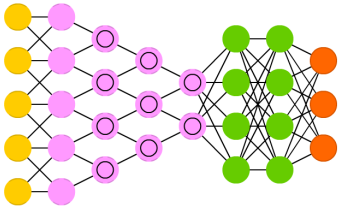
\includegraphics[scale=1]{media_tesi/DCN.png}} \\
\vspace{2cm}
\subfloat[][\emph{una GAN}]
{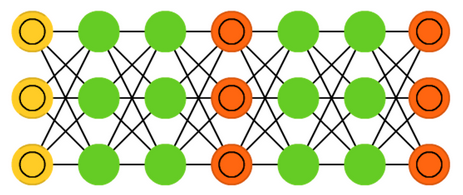
\includegraphics[scale=0.7]{media_tesi/GAN.png}} \\
\vspace{2cm}
\subfloat[][\emph{una RNN}]
{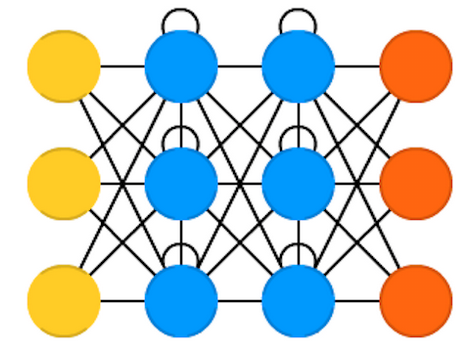
\includegraphics[scale=0.4]{media_tesi/RNN.png}}\\

\label{fig:subfig}
\end{figure}